\documentclass[letterpaper, reqno,11pt]{article}
\usepackage[margin=1.0in]{geometry}
\usepackage{color,latexsym,amsmath,amssymb,graphicx,float,listings,tikz}
\usepackage{hyperref}

\hypersetup{
colorlinks=true,
linkcolor=magenta,
filecolor=magenta,
urlcolor=cyan,
}

\graphicspath{ {images/} }

\begin{document}
\pagenumbering{arabic}
\title{Math 318 Homework 7}
\date{16/03/23}
\author{Xander Naumenko}
\maketitle

{\medskip\noindent\bf Question 1a.} The definition of a characteristic function is $\phi_{X}(t)=E[e^{itX}]$. Expanding this, we get: 
\[
\phi_{X}(t)=E[e^{itX}]=\int_{-\infty}^{\infty}f_X(x) e^{itx}dx=\sum_{x=-\infty}^{\infty}p_X(x) e^{itx}=\sum_{x=-\infty}^{\infty}p_X(x) \left( \cos(tx)+i\sin(tx) \right) 
.\]
The only $t$ dependence is in the $\sin(tx)$ and $\cos(tx)$ terms which are both $2\pi$ periodic (since $x$ is an integer), so the characteristic function of discrete variables is $2\pi$-periodic. 

% {\medskip\noindent\bf Question 1b.} Let $Y=$

% \[
%     E[Y]=\frac{1}{i}\phi_Y'(0)=\int_{-\infty}^{\infty}yf_Y(y)dy=\frac{1}{i}\phi_Y'(2\pi)=\int_{-\infty}^{\infty}yf_Y(y)e^{2\pi iy}dy
% .\]
% \[
% \phi_X(0)=\int_{-\infty}^{\infty}f_X(x)dx=\phi_X(2\pi)=\int_{-\infty}^{\infty}f_X(x)e^{2\pi ix}dx
% .\]

{\medskip\noindent\bf Question 1b.} Consider $\phi(2\pi)$. By definition and the periodicity of $X$, this is
\[
    \phi(2\pi)=E[e^{2\pi iX}]=\phi(0)=\int_{-\infty}^{\infty}f_X(x)dx=1
.\]
However the only way that $e^{2\pi iX}=1$ ever occurs is if $X$ is an integer. If there is a nonzero probability $X$ is ever a non-integer, the real part of the expected value would be $\text{Re}[e^{2\pi iX}]=\cos 2\pi X<1(\text{for } X \not\in \mathbb{Z})$, which would cause the expected value to be less than 1. Thus is must be that $X\in\mathbb{Z}$ with probability 1. 

{\medskip\noindent\bf Question 2.} Expressing as an integral: 
\[
    E[X^3]=\int_{-\infty}^{\infty}\int_{-\infty}^{\infty}(u+v)^3f_U(u)f_V(v)dudv=\iint (u^3+3u^2v+3uv^2+v^3)f_U(u)f_V(v)dudv
\]
\[
    =E[U^3]+E[V^3]+3E[U^2]E[V]+3E[U]E[V^2]=E[U^3]+E[V^3]
.\]
Similarly for $E[X^{4}]$: 
\[
    E[X^4]=\int_{-\infty}^{\infty}\int_{-\infty}^{\infty}(u+v)^4f_U(u)f_V(v)dudv=\iint (u^4+4u^3v+6u^2v^2+4uv^3+v^3)f_U(u)f_V(v)dudv
.\]
\[
    =E[U^4]+E[V^4]+6E[U^2]E[V^2]+4E[U^3]E[V]+4E[U]E[V^3]=E[U^4]+E[V^4]+6E[U^2]E[V^2]
.\]

{\medskip\noindent\bf Question 3a.} Let the entries of $A$ be denoted by $A_{ik}$, where $i$ is the row and $k$ is the column. Then by the definition of matrix multiplication,
\[
    Y_i=\sum_{k=1}^{n}A_{ik}X_k
.\]
The distribution of a sum of normal variables is also a normal variable with the sum of mean and variance added, so $Y_i=N(0,n)$. 

{\medskip\noindent\bf Question 3b.} Computing covariance
\[
    \text{Cov}(Y_i,Y_j)=E[Y_iY_j]-E[Y_i]E[Y_j]=E\left[\left(\sum_{k=1}^{n}A_{ik}X_k\right)\left( \sum_{k=1}^{n}A_{jk}X_k \right) \right]
\]
\[
    =E\left[\sum_{k=1}^{n}\sum_{l=1}^{n}A_{ik}A_{jl}X_kX_l\right]=\sum_{k=1}^{n}\sum_{l=1}^{n}A_{ik}A_{jl}E[X_kX_l]=\sum_{k=1}^{n}A_{ik}A_{jk}E[X_k^2]
\]
\[
=A_i\cdot A_j
\]
where $A_i$ and $A_j$ are the $i$th and $j$th row vector of $A$ respectively.

{\medskip\noindent\bf Question 3c.} We will prove the general case of the bonus problem, and $n=2$ is just a special case. Since $Y=AX$ is linear, the Jacobian is just $J=A$. Since each of the $X_i$s are independent, their joint probability distribution function is (using explicit vector notation on lower case $\vec x$/$\vec y$ for clarity)
\[
    f_X(\vec x)=\prod_{i=1}^{n}f_{X_i}(x_i)=\prod_{i=1}^{n}\frac{1}{\sqrt{2\pi} }e^{x_i^2 /2}=\frac{1}{(2\pi)^{n/2}}e^{(\vec x\cdot\vec x)/2}=\frac{1}{(2\pi)^{n/2}}e^{(\vec x^{T}\vec x)/2}
.\]
Thus using the Jacobian we have
\[
f_Y(\vec y)=\frac{1}{|J|}f_X\left( A^{-1}\vec y \right)=\frac{1}{(2\pi)^{n /2}|\det A|}e^{-\left( \vec y^{T}A^{T-1}A^{-1}\vec y \right) /2}
.\]
This is what was desired, so we're done. As mentioned, for the non-bonus problem, simply apply this to $n=2$. 

{\medskip\noindent\bf Question 4.} For the following sections this code was used to generate the figures:

\begin{lstlisting}
import numpy as np
import random
import matplotlib.pyplot as plt
from tqdm import tqdm

n = 1000000
sims = 1000
ps = (0.5, 0.51, 0.502)

figa, axa = plt.subplots(3)
for j, p in enumerate(ps):
    X = [0]
    for i in range(n-1):
        X.append(X[i] + (-1 if random.random() > p else 1))
        
    axa[j].plot(list(range(n)), X)
    axa[j].set_title(f'p={p}')

plt.show()

figb, axb = plt.subplots(3)
figc, axc = plt.subplots(3)
for j, p in enumerate(ps):
    T = np.array([n]*sims)
    for sim in tqdm(range(sims)):
        X = 0
        for t in range(n):
            X += -1 if random.random() > p else 1
            if X == 0:
                T[sim] = t
                break

    axb[j].hist(T, bins=np.arange(0, n + 10000, 10000))
    axb[j].set_title(f'p={p}')

    T.sort()
    F = []
    s = 0
    for t in range(n):
        while s < len(T) and T[s] <= t:
            s += 1
        F.append((sims-s)/sims)

    axc[j].loglog(np.arange(n), F)
    axc[j].set_title(f'p={p}')
    print(sum(T)/len(T))
    print(sum(T), len(T))

plt.show()
\end{lstlisting}

{\medskip\noindent\bf Question 4a.} See figure \ref{fig:4a}. 

\begin{figure}[htpb]
    \centering
    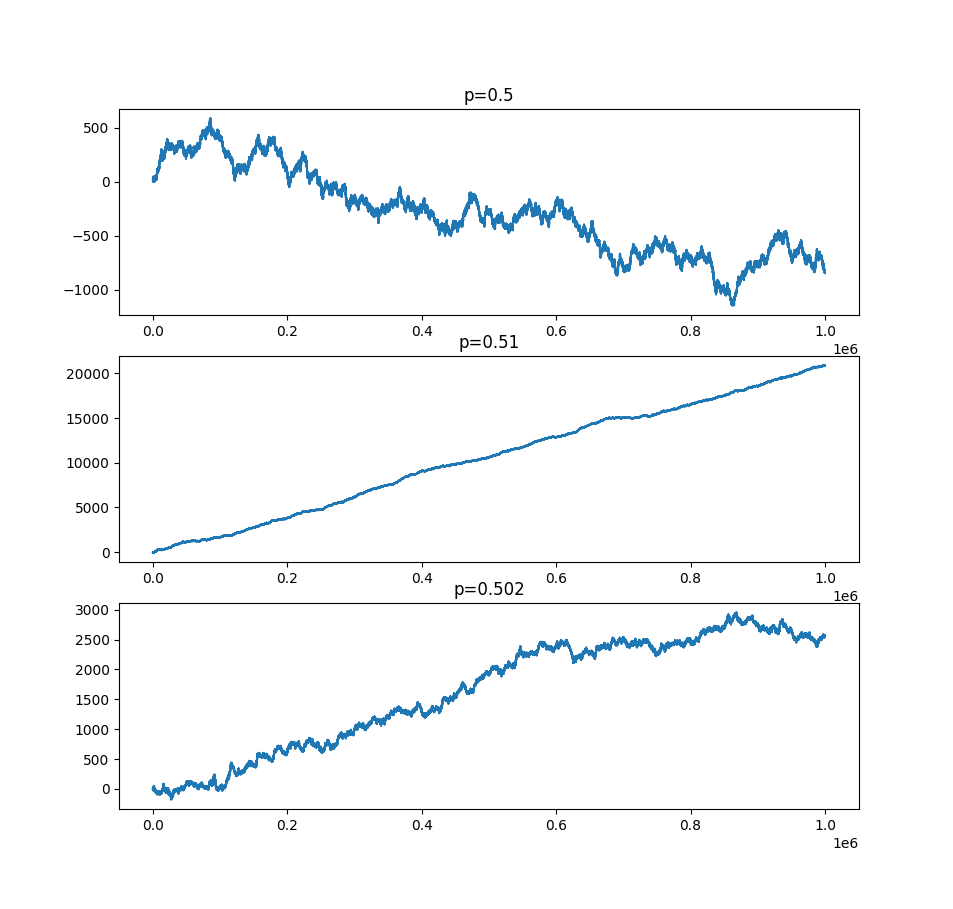
\includegraphics[width=0.8\textwidth]{4a}
    \caption{Graph for question 4a.}
    \label{fig:4a}
\end{figure}

{\medskip\noindent\bf Question 4b.} See figure \ref{fig:4b}. Of the walks, 1 didn't return for $p=0.5$, 17 didn't return for $p=0.51$ and 5 didn't return for $p=0.502$

\begin{figure}[htpb]
    \centering
    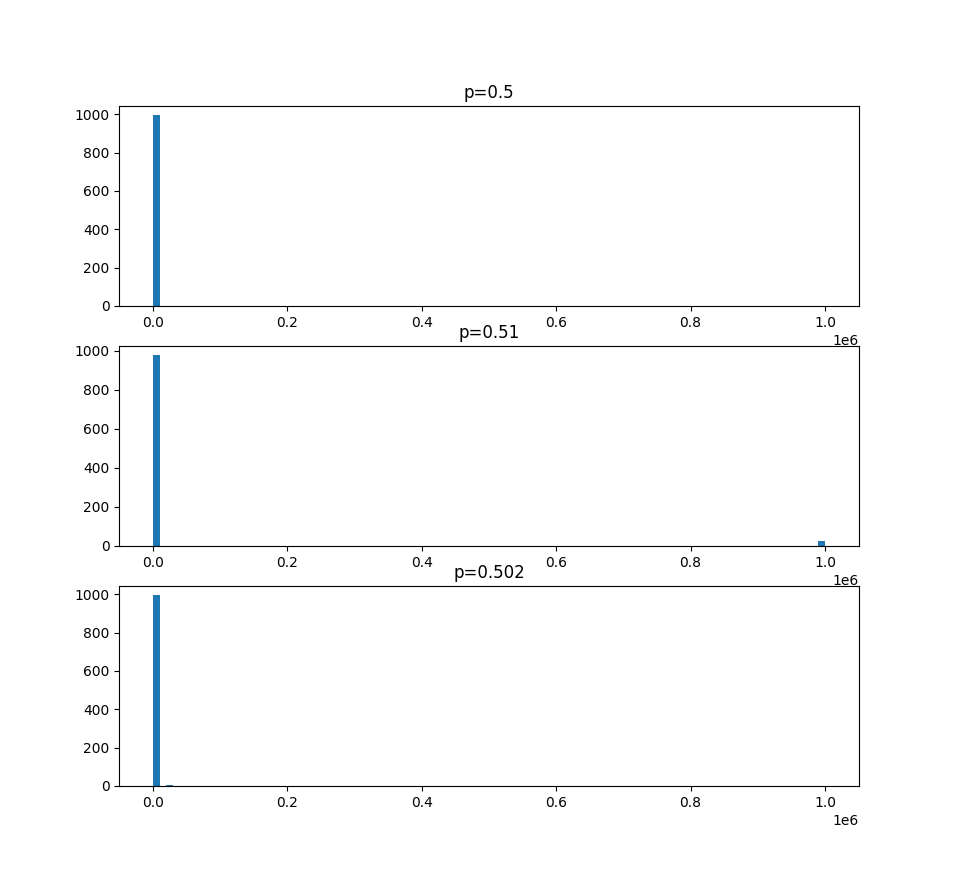
\includegraphics[width=0.8\textwidth]{4b}
    \caption{Histogram for question 4b.}
    \label{fig:4b}
\end{figure}

{\medskip\noindent\bf Question 4c.} See figure \ref{fig:4c}.

\begin{figure}[htpb]
    \centering
    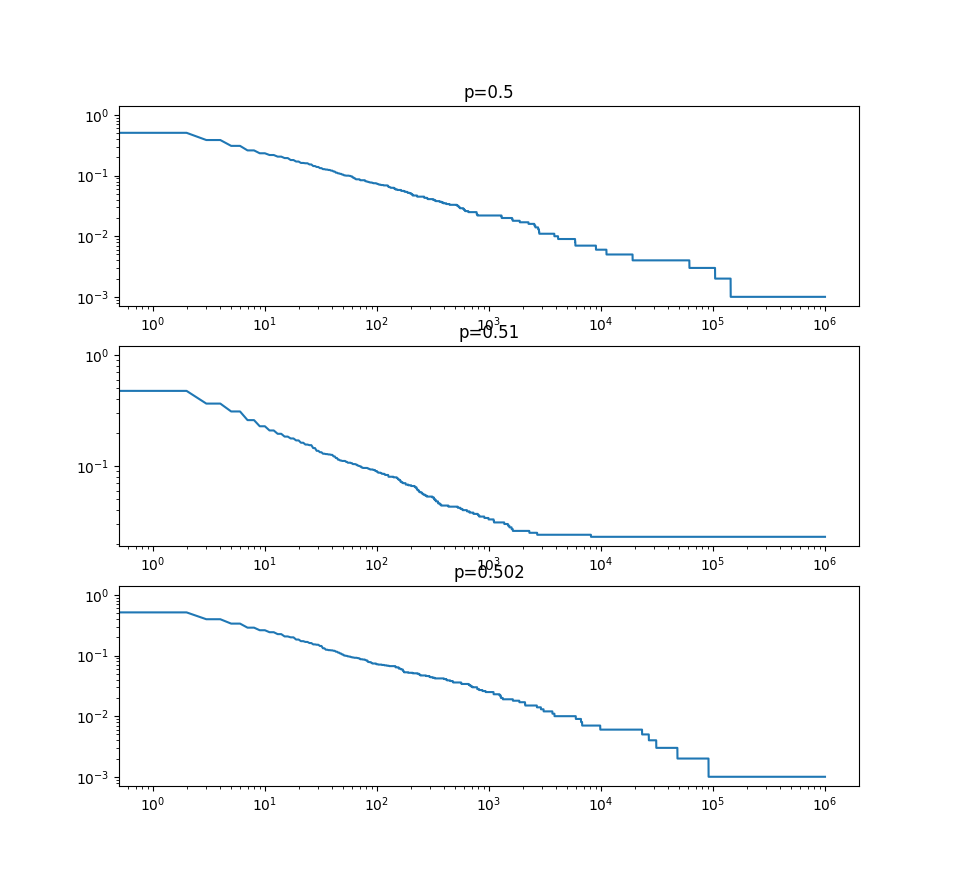
\includegraphics[width=0.8\textwidth]{4c}
    \caption{Graphs for question 4c.}
    \label{fig:4c}
\end{figure}

{\medskip\noindent\bf Question 4d.} From the plots it seems that $P(T>n)=0$ as $n\to \infty$. It seems from the plots that they settle down to 0. Calculating the means from the data they were 2340, 26066 and 3163 respectively. The unbiased random walk is recurrent, so if there was no termination it would be larger than we see but still finite. Biased walks were proved in class to have infinite mean, so I would expect their mean to grow to infinity with no limit. 

{\medskip\noindent\bf Question 5.} The following code was used for this question: 
\begin{lstlisting}
import numpy as np
import matplotlib.pyplot as plt
import random
from tqdm import tqdm

n = 1000000
sims = 1000
directions = [np.array(d) for d in [(1, 0), (0, 1), (-1, 0), (0, -1)]]

S = np.empty((n, 2))

for i in range(n-1):
    S[i+1] = S[i] + random.sample(directions, 1)

plt.scatter(S.T[0], S.T[1], c=np.arange(0, n), cmap="rainbow", s=0.2)

plt.show()


n_steps = []
for sim in tqdm(range(sims)):
    S = np.empty((n, 2))

    n_steps.append(n)
    for i in range(n-1):
        S[i+1] = S[i] + random.sample(directions, 1)
        if S[i+1][0] == 0 and S[i+1][1] == 0:
            n_steps[-1] = i+1
            break

plt.hist(n_steps)

print(n_steps)
print(len([x for x in n_steps if x == n]))

plt.show()
\end{lstlisting}

{\medskip\noindent\bf Question 5a.} See figure \ref{fig:5a}

\begin{figure}[htpb]
    \centering
    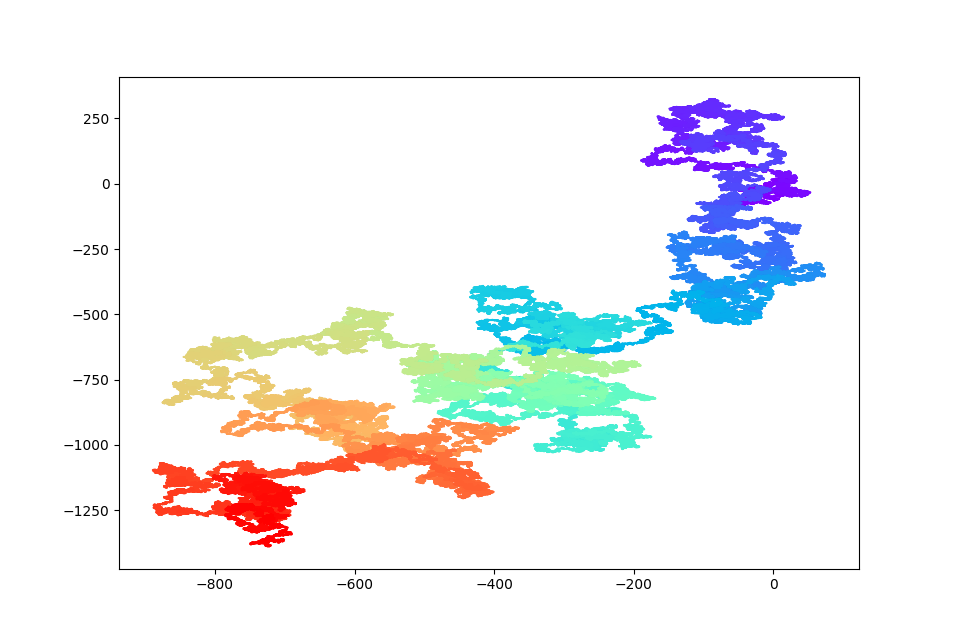
\includegraphics[width=0.8\textwidth]{5a}
    \caption{Scatter plot for 5a.}
    \label{fig:5a}
\end{figure}

{\medskip\noindent\bf Question 5b.} The number of walks that failed to return to 0 is 305, which is obviously quite high. This is consistent with the fact that random walks are recurrent though, as we are terminating the walks at a finite threshold, in an infinite random walk it is guaranteed to be recurrent.

{\medskip\noindent\bf Question 5c.} See figure \ref{fig:5b}.

\begin{figure}[htpb]
    \centering
    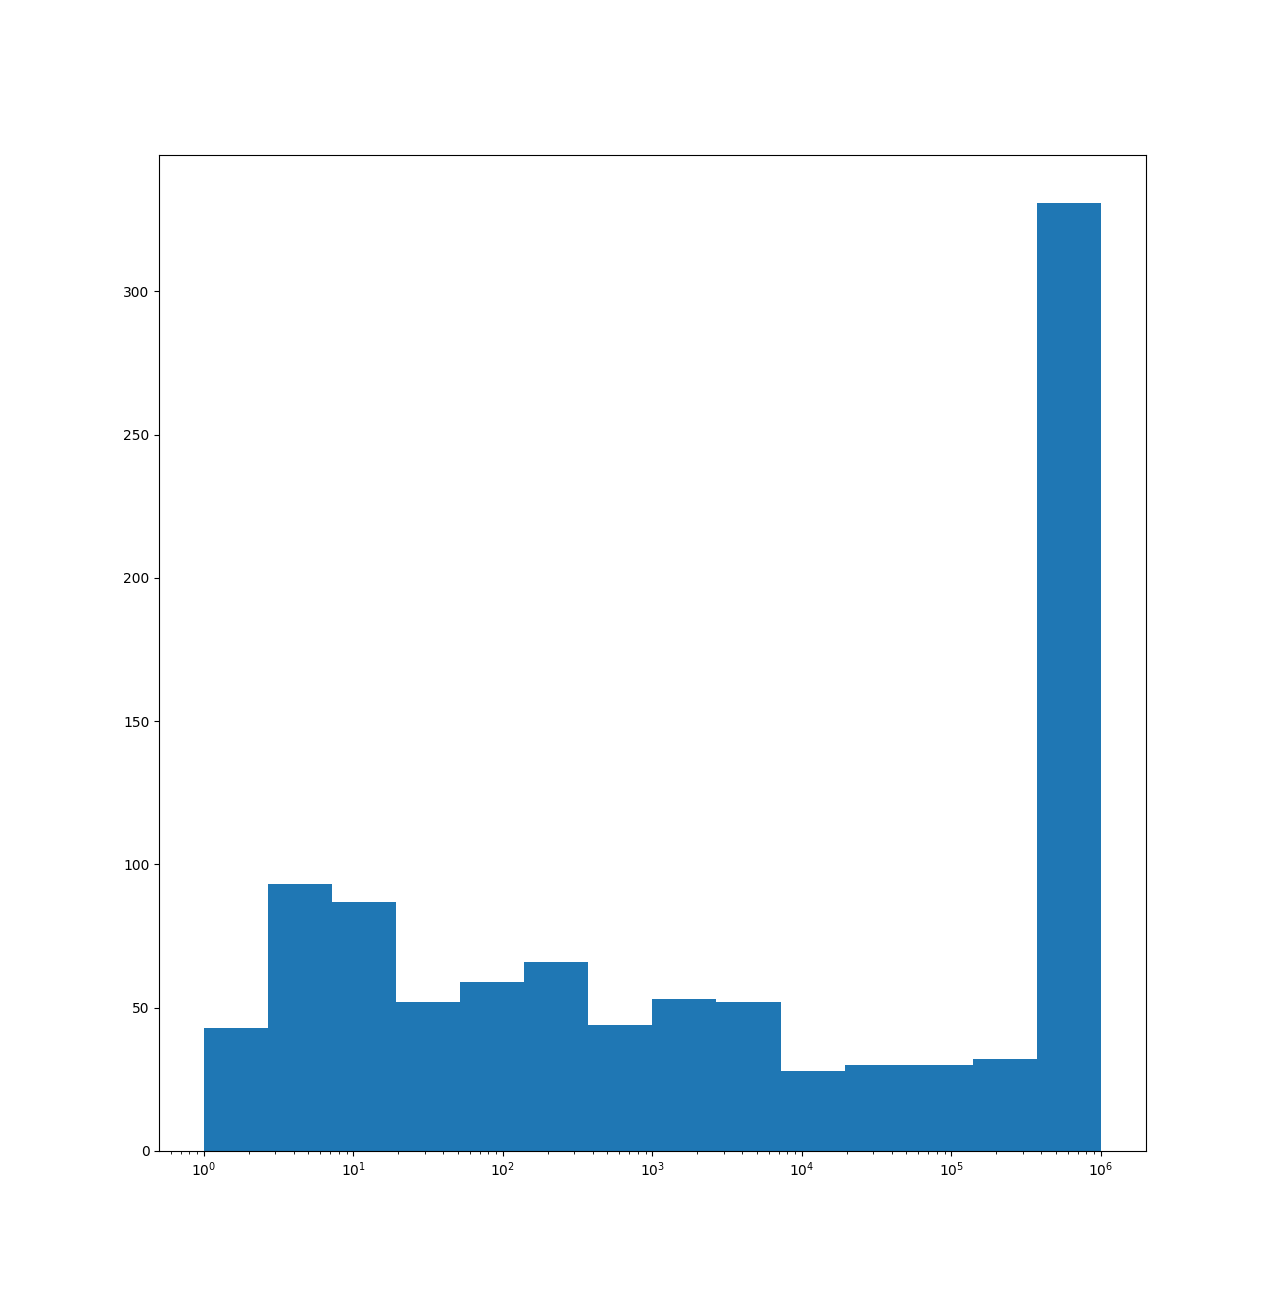
\includegraphics[width=0.8\textwidth]{5b}
    \caption{Histogram for question 5b.}
    \label{fig:5b}
\end{figure}

\end{document}
